\subsubsection{Screen Flow}

\begin{figure}[H] % Sửa htbp thành H để khóa chặt vị trí ảnh
    \centering
    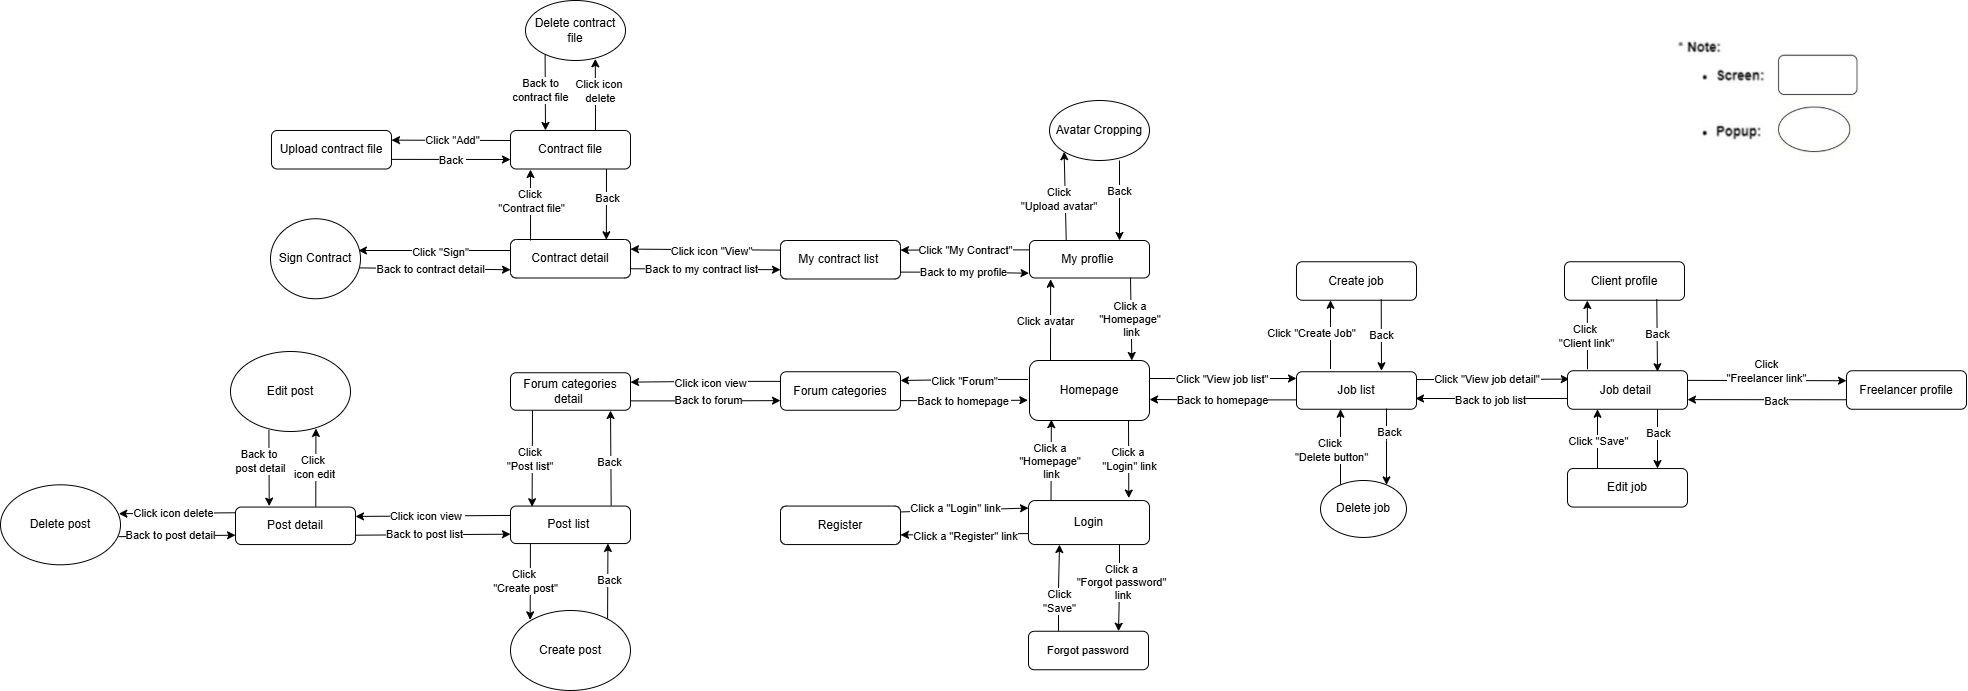
\includegraphics[width=\linewidth]{image/Screen_flow/Screen_flow_for_client.drawio.png}
    \caption{Screen Flow of Client}
    \label{fig:screenflowclient}
\end{figure}

\begin{figure}[H] % Sửa htbp thành H
    \centering
    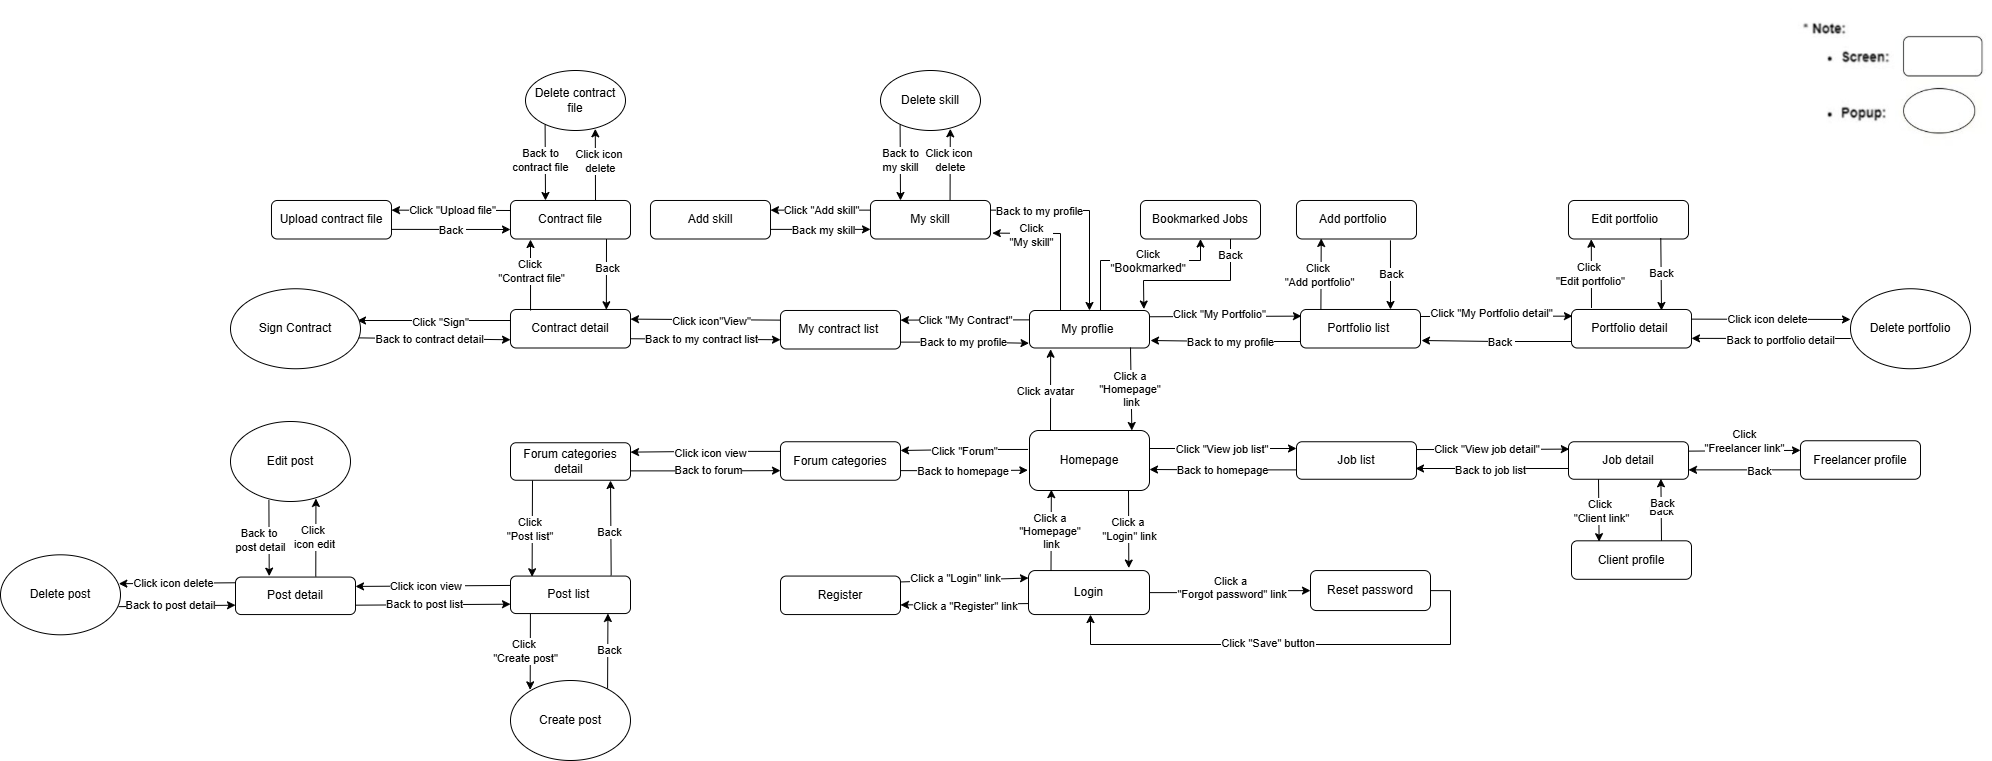
\includegraphics[width=\linewidth]{image/Screen_flow/Screen_flow_for_freelancer.drawio.png}
    \caption{Screen Flow of Freelancer}
    \label{fig:screenflowfreelancer}
\end{figure}

\begin{figure}[H] % Sửa htbp thành H
    \centering
    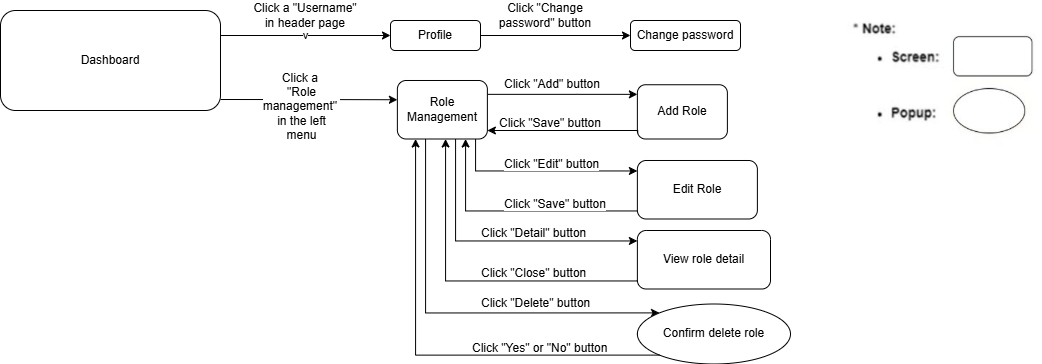
\includegraphics[width=\linewidth]{image/Screen_flow/Screen_flow_for_admin.drawio.png}
    \caption{Screen Flow of Admin}
    \label{fig:screenflowadmin}
\end{figure}

\begin{figure}[H] % Sửa htbp thành H
    \centering
    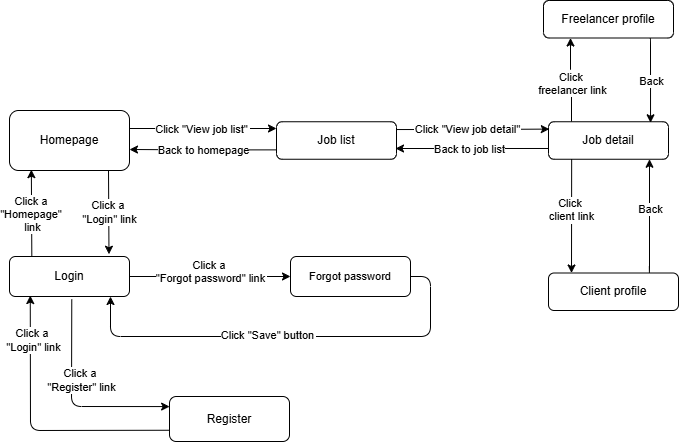
\includegraphics[width=\linewidth]{image/Screen_flow/Screen_flow_for_guest.drawio.png}
    \caption{Screen Flow of Guest}
    \label{fig:screenflowguest}
\end{figure}

% Ngắt trang bắt buộc để phần Bảng bên dưới sang trang mới sạch sẽ, không bị dính vào ảnh
\clearpage